\chapter{About Wave-DNA}
\label{chap:About Wave-DNA}

\section{Purpose}
\label{sec:Purpose}

{\tt Wave-DNA} is a simulation tool for one-dimensional and spherically symmetric nonlinear acoustic waves in transient and spatially variable background flow fields. The motion of the background medium is accounted for by considering a convective form of the lossless Kuznetsov wave equation, derived from the first principles based on perturbations of the continuity equation and the transient Bernoulli equation. The method is optimized for boundary value problems. The background flow field, in which the acoustic wave propagates, is treated as an input to the wave solver. In principle, the background flow field my be obtained from analytical considerations, numerical simulations, or experimental measurements.

The moving boundary may represent a moving wave emitter or scatterer, and it may move relative to the medium or displace the surrounding fluid. This allows the user to study nonlinear Doppler effects associated with moving wave emitters/scatterers and/or non-uniform background accelerating flow fields. The motion of the domain boundary is conveniently taken into account by a generic coordinate transformation of the governing wave equation, where the transformed wave equation is solved in a fixed computational domain. This technique enables accurate numerical solutions of the combined wave-flow problem without the necessity to interpolate data between the moving grid points in the physical domain. The numerical technique is based on explicit finite differences, and it is equipped with a predictor-corrector method to counteract the onset and growth of dispersive numerical noise in the cases of broad frequency bands or shock formation. Furthermore, absorbing boundary conditions can be imposed in order to let the acoustic waves pass the domain boundaries without reflection.

A particularly well-suited example to demonstrate the capability of the simulation framework is the so-called acoustic black/white hole analogy as presented in [REF]. The present documentation provides detailed instructions on how to reproduce the acoustic black/white hole simulations in [REF] using {\tt Wave-DNA}, as well as other examples to demonstrate the capabilities and functionalities of the tool.

It is important to note that rather than representing compressible background flow fields with variable $\rho_0$ and $c_0$, the acoustic black/white hole configurations are model systems for acoustic waves propagating in accelerating flow fields of any (also subsonic) velocity magnitude. The reason for the acoustic black/white hole being such a convenient system for the computational study of acoustic waves in accelerating flow fields lies in the fact that they allow to trap a wave characteristic at the point of sonic transition, the sonic horizon, where it is subject to both a constant background flow velocity and a constant background flow acceleration. Due to the nonzero acceleration, the neighbouring characteristics are either converging towards or diverging away from the sonic horizon.





\section{Underlying theory}
\label{sec:Underlying theory}

The theoretical framework is based on a previously derived lossless and quasi one-dimensional convective form of the Kuznetsov equation for planar waves and curved wavefronts with variable cross-sectional area $A$, i.e.
\begin{equation}
\left(1 + \dfrac{2\beta - 1}{c_0^2}\dfrac{\mathrm{D}\phi_1}{\mathrm{D}t}\right)\dfrac{\mathrm{D}^2\phi_1}{\mathrm{D}t^2}
- c_0^2\left(\dfrac{\partial^2}{\partial r^2} + \dfrac{1}{A}\dfrac{\partial A}{\partial
r}\dfrac{\partial}{\partial r}\right)\phi_1
+ \dfrac{1}{\rho_0}\dfrac{\mathrm{D}\mathcal{L}}{\mathrm{D}t}
+ \dfrac{\partial \phi_1}{\partial r}\dfrac{\partial}{\partial r}\left(\dfrac{\mathrm{D}\phi_1}{\mathrm{D}t}\right) = 0,
\label{eq:convectiveKuznetsov}
\end{equation}
where $\phi_1$ is the acoustic velocity potential. The equation is derived based on a perturbation of the continuity equation and the transient Bernoulli equation. In this framework, the subscript ``0'' indicates the background state and ``1'' the acoustic perturbation. In particular, the density $\rho_0$ and the speed of sound $c_0$ act as constant background quantities. The derivation of the wave equation points towards an extension to variable background state variables, which, however, would generate additional terms that are neglected here. The material derivative operator is defined based on the background flow velocity $u_0$, i.e.
\begin{equation}
\dfrac{\mathrm{D}}{\mathrm{D}t} = \dfrac{\partial}{\partial t} + u_0 \dfrac{\partial}{\partial r}.
\label{eq:MaterialDerivative}
\end{equation}
The background flow velocity $u_0\left(r,t\right)$ can be both time-dependent and spatially non-uniform. However, one should only be confident about the accuracy of Eq. \eqref{eq:convectiveKuznetsov} if $u_0$ varies slowly on the length and time scales of the acoustic wave \citep{Pierce_1990}. The transient Bernoulli equation provides the relation
\begin{equation}
\dfrac{p_1}{\rho_0} = - \dfrac{\mathrm{D}\phi_1}{\mathrm{D}t} - \dfrac{\mathcal{L}}{\rho_0} - \dfrac{\beta - 1}{c_0^2}\left(\dfrac{\mathrm{D}\phi_1}{\mathrm{D}t}\right)^2,
\label{eq:p1pi1}
\end{equation}
which is needed to convert between the perturbation potential $\phi_1$ and the acoustic pressure $p_1$.

Eq. \eqref{eq:convectiveKuznetsov} admits two sources of nonlinear wave propagation. One is related to the nonlinearity coefficient $\beta$ and manifests in cumulative wave-steepening and shock formation at high amplitudes, where the nonlinearity coefficient beta $\beta$ is representative of how strongly the local speed of sound is modified by the acoustic pressure. The second source of nonlinearity stems from a non-zero Lagrangian density \citep{Zhong_et_al_2021}
\begin{equation}
\mathcal{L} = \dfrac{1}{2}\rho_0u_1^2 - \dfrac{1}{2}\dfrac{p_1^2}{\rho_0 c_0^2}
\label{eq:LagrangianDensity},
\end{equation}
giving rise to locally nonlinear behavior as the linear acoustic relation $p_1 = \rho_0 c_0 u_1$ breaks down \citep{Cervenka_and_Bednarik_2022}. For $\mathcal{L}=0$, Eq. \eqref{eq:convectiveKuznetsov} reduces to the lossless convective Westervelt equation. If both $\mathcal{L}=0$ and $\beta=0$, the convective wave equation is obtained \citep{Pierce_1990, Kaltenbacher_and_Hueppe_2018}.

In order to represent moving domain boundaries and deforming physical domain, the time-dependent coordinate transformation
\begin{equation}
r: \: \left[\mathcal{X}_R,\mathcal{X}_{\infty}\right]
\rightarrow \left[R\left(t\right),r_{\infty}\right], \: \left(\xi,t\right) \mapsto r\left(\xi,t\right)
\label{eq:coordTrans}
\end{equation}
is invoked, which yields
$\phi_1\left(r\left(\xi,t\right),t\right)=\Phi_1\left(\xi,t\right)$ and, therefore \citep{Schenke_et_al_2022},
\begin{align}
& \dfrac{\partial^k \phi_1}{\partial r^k} = \left(\dfrac{\partial \xi}{\partial r} \dfrac{\partial}{\partial \xi}\right)^k\Phi_1,
\label{eq:transDerivativeOp_space} \\
& \dfrac{\partial^k \phi_1}{\partial t^k} = \left(\dfrac{\partial \xi}{\partial t} \dfrac{\partial}{\partial \xi} + \dfrac{\partial}{\partial t}\right)^k\Phi_1.
\label{eq:transDerivativeOp_time}
\end{align}
Due to Eqs. \eqref{eq:transDerivativeOp_space} and \eqref{eq:transDerivativeOp_time}, additional terms are generated in the computational domain with coordinates $\left(\xi, t\right)$, in which the transformed governing equation is discretized and solved as illustrated by Fig. \ref{fig:domains}. The derivation of the transformed wave equation is provided in Appx. \ref{chap:Appendix}.


\begin{figure}
{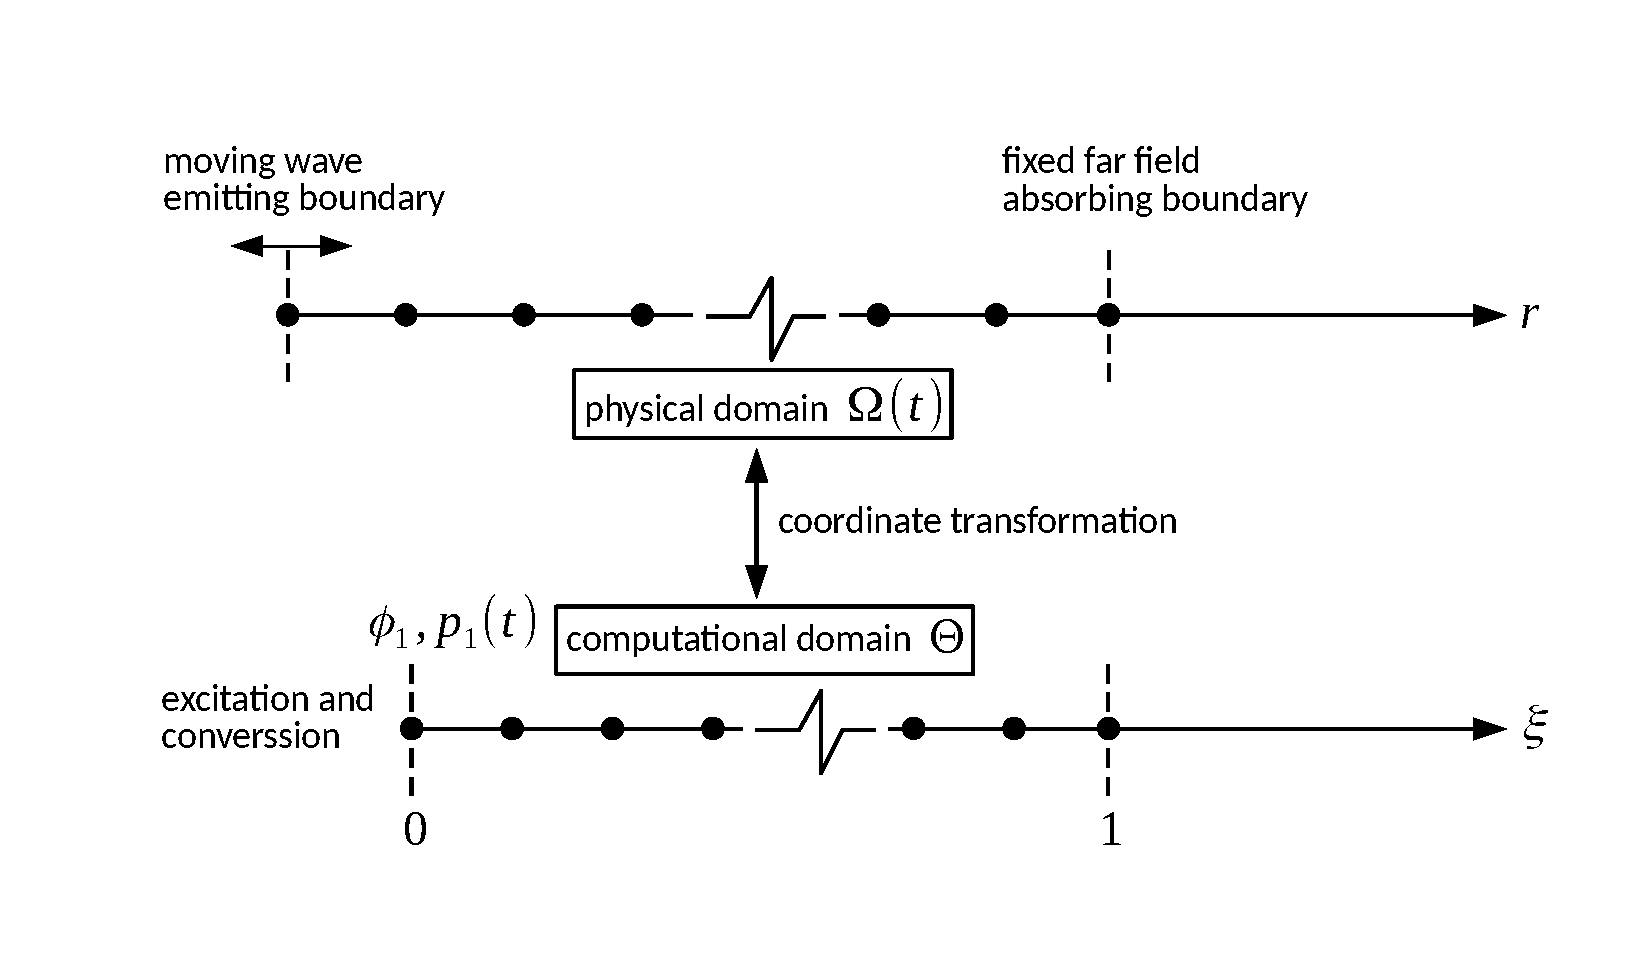
\includegraphics[width=0.8\textwidth]{figures/domains.pdf}}
\caption{Schematic of the physical domain $\Omega\left(t\right)$, with moving wave-emitting boundary and fixed wave absorbing boundary, and the fixed computational domain $\Theta$. The coordinate transformation specifies a mapping between the domains.}
\label{fig:domains}
\end{figure}


\section{Importance of the coordinate transformation}
\label{sec:Importance of the coordinate transformation}

The coordinate transformation is not only a convenient means to model the moving domain boundary. In the acoustic black/white hole scenario, it also plays a key role in establishing a well-posed formulation of the governing wave equation.

The importance of the coordinate transformation can be illustrated at the example of the standard convective wave equation of the form $\mathrm{D}^2\phi_1/\mathrm{D}t^2 = c_0^2\partial^2\phi_1/\partial x^2$ with material derivative operator $\mathrm{D}/\mathrm{D}t = \partial/\partial t + u_0\partial/\partial x$. This equation is easily shown to loose its well-posedness as $u_0$ approaches the sonic speed $c_0$. This is because the second material derivative generates another Laplacian term with coefficient $u_0^2$ so that the Laplacian coefficient effectively becomes $c_0^2-u_0^2$ and changes its sign as $u_0$ exceeds the sonic speed, thus rendering the equation ill-posed. With the coordinate transformation, which can be seen as a Galilean-type transformation in physical space, this problem is circumvented by locally switching into a reference frame that moves, at least approximately, along with the fluid flow. This has the effect that the additional terms arising from the coordinate transformation preserve the sign of the Laplacian coefficient.
